% Explain the atomic island concept
% Inter atomic-island switches
% Explain how this will be the grid we'll be optimizing on
% Explain that we can merge in the atomic islands acting as "leafs" (show comparison graph)grid
% Explain the problem with not connected parts of the grid in the satandard switch case and the solution

To test out different gird configurations some data preparation is required. The following
steps will be showcased utilizing an anonymized grid topology of one of Venios' customers. 
The specific grid data comes from a Swiss suburb. The data has been loaded through the api calls
described previously. This was done by choosing a geographical bounding box and obtaining grid
data for all grids contained.\\
The more grids, components and switches are in an area the more switch states are possible
and the less likely it is to find optimal switch states for the entire area. For this example
a grid area with the following elements was chosen:

\begin{figure}[H]
    \begin{center}
        \begin{tabular}{ll}
            Grids & 5\\
            Nodes (all types) & 2890\\
            Edges (all types) & 2958\\
            Transformer & 10\\
            Cables & 1995\\
            Prosumers & 600\\
            Switches & 152\\
        \end{tabular}
    \end{center}
    \caption{
        Number of grid elements in the chosen example grid area within a Swiss suburb.
    }
    \label{table:data_prep:swiss_suburban_numbers}
\end{figure}

\subsection{Atomic islands}

In a first step what will here be called atomic islands have to be formed. Figure \ref{fig:data_prep:atomic_islands}
shows some arbitrary grid topology with some nodes and edges. Atomic islands are clusters
of nodes and edges which can not be subdivided by switches further. In the example shown
it is easy to see that two non-divisible clusters can be formed. One containing nodes
1 to 4 and one containing nodes 5 to 8.

\begin{figure}[H]
    \begin{center}
        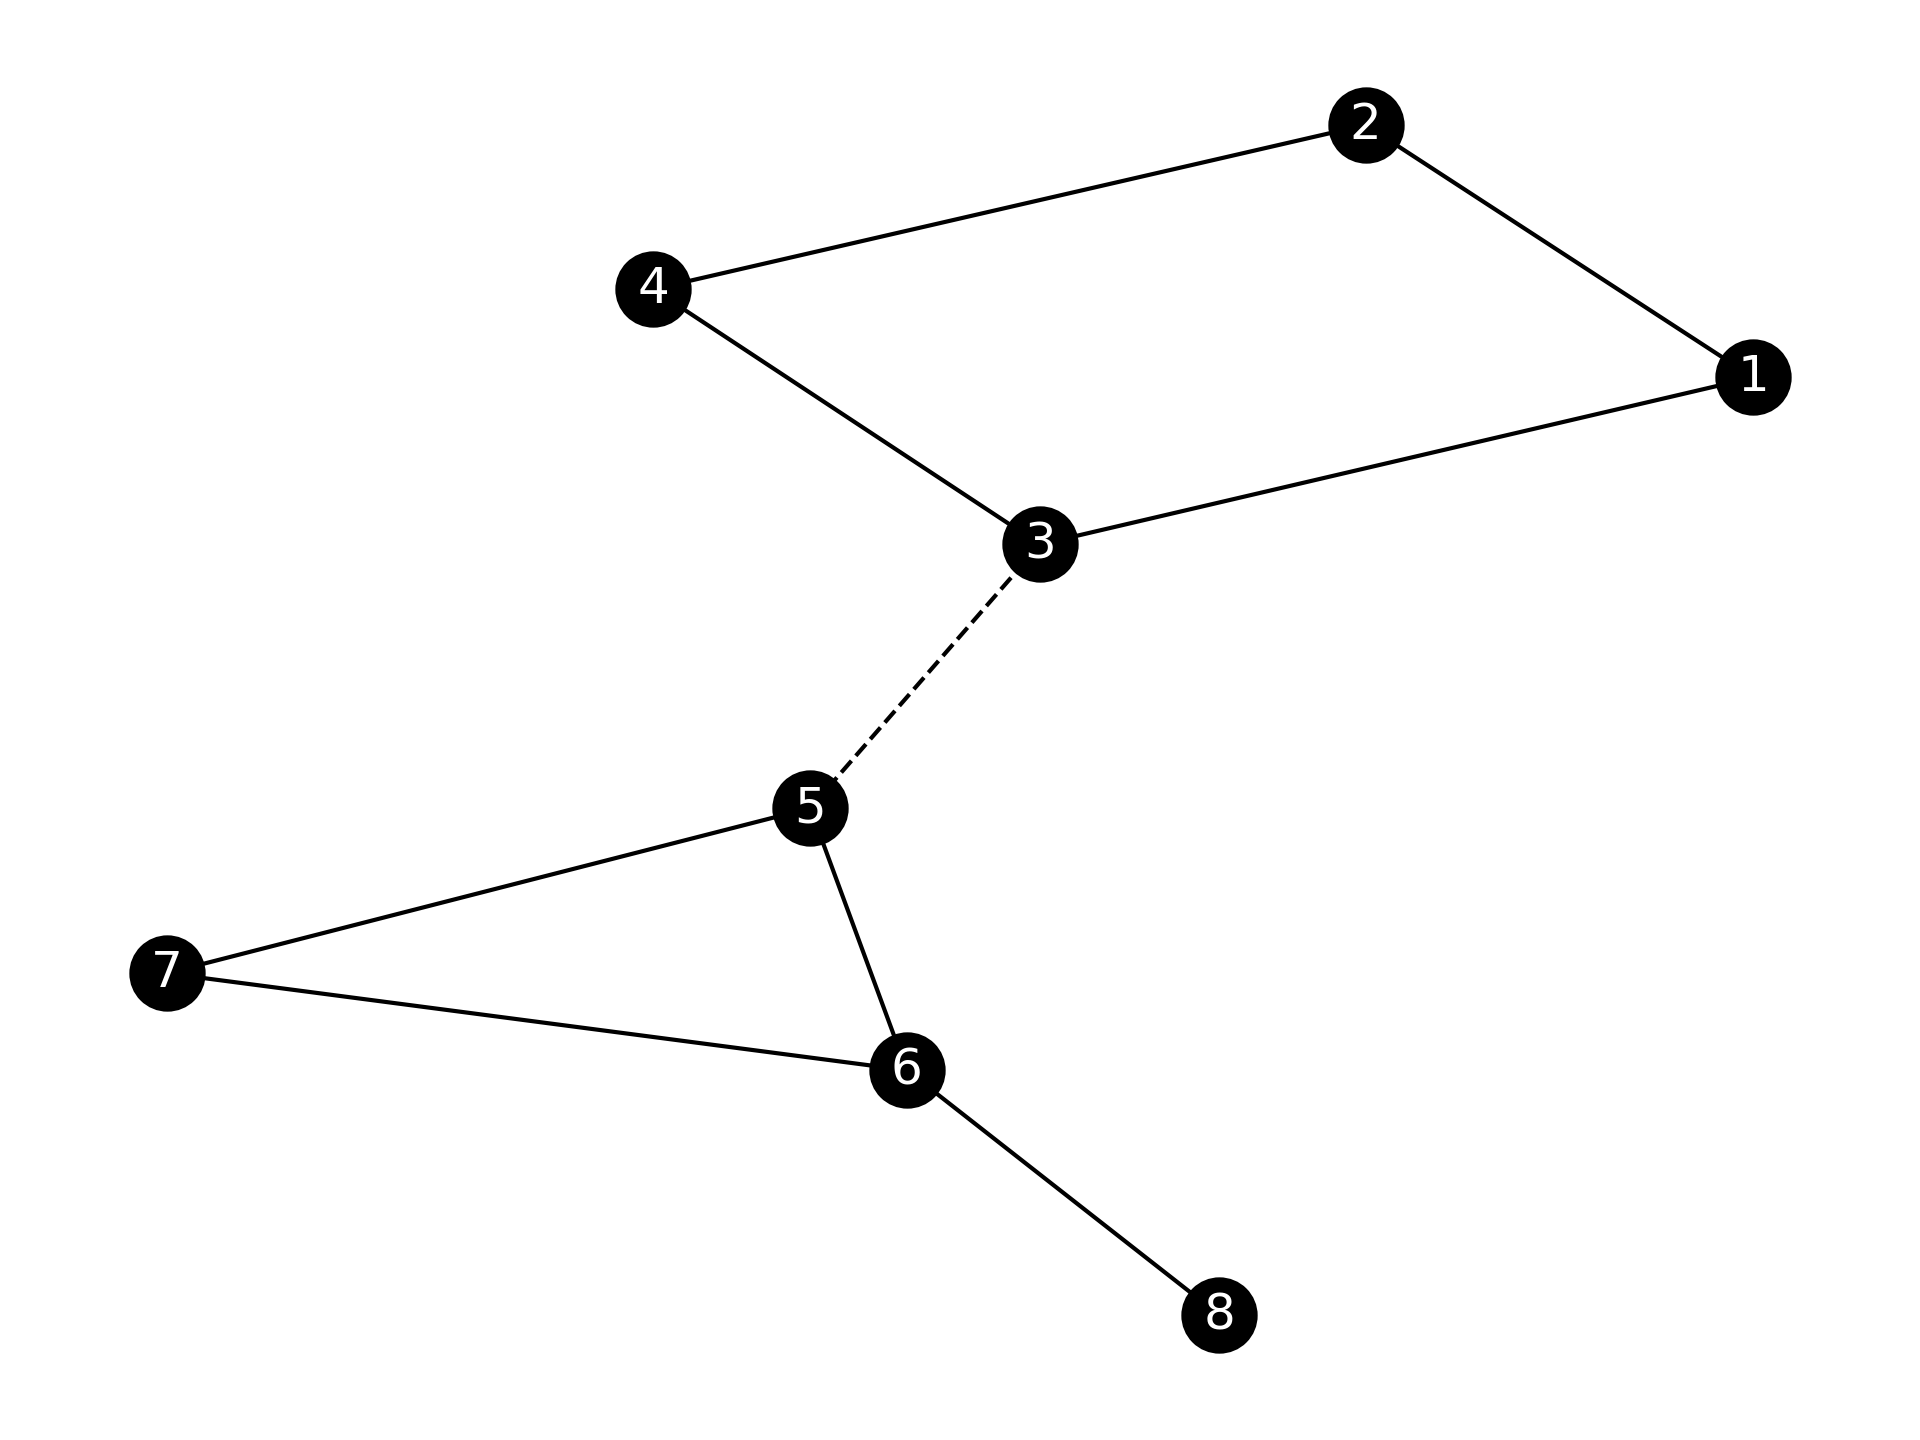
\includegraphics[width=.7\linewidth]{img/atomic_island.png}
    \end{center}
    \caption{
        Example grid topology with 8 nodes and 9 edges. Switches
        are drawn as a dashed line
    }
    \label{fig:data_prep:atomic_islands}
\end{figure}

To do this algorithmically the edges are considered in edge list
form (\ref{eq:graph_theory:edge_list}). They can then be iterated over.
The nodes are initially put into their own atomic island by themselves.
For each edge that is not a switch, each of the atomic islands on either
side are merged:


\begin{algorithm}[h!]
    \SetKw{New}{new}
    \SetKwFunction{Dict}{Dict}


    $I \gets $ \{\}\;
    $island\_of\_node \gets $ \New \Dict{}\;

    \ForEach{$i < N$}{
        $I_i \gets $  \{ $i$ \}\;
        $I \gets I \cup \{I_i$\}\;
        $island\_of\_node[i] \gets I_i$\;
    }

    \ForEach{$(i, j) \in edges \setminus switches$}{

        $I \gets I \setminus {island\_of\_node[i]}$\;
        $I \gets I \setminus {island\_of\_node[j]}$\;
        $M \gets island\_of\_node[i] \cup island\_of\_node[j]$\;

        \ForEach{$k \in M$}{
            $island\_of\_node[i] \gets M$\;
        }

        $I \gets I \cup \{M$\}\;
    }
    
    \caption{Algorithm to obtain atomic islands}
    \label{alg:data_prep:atomic_islands}
\end{algorithm}

This algorithm yields the atomic islands, represented as a set of node indices.\\
Its worth noting that this algorithm can be used for any kind of island formation,
it will come in useful again later when different forms of islands need constructing.\\

Applying this procedure to the grid mentioned in table \ref{table:data_prep:swiss_suburban_numbers},
produces an atomic island structure depicted in figure \ref{fig:data_prep:swiss_suburb_with_leafs}.

\begin{figure}[H]
    \begin{center}
        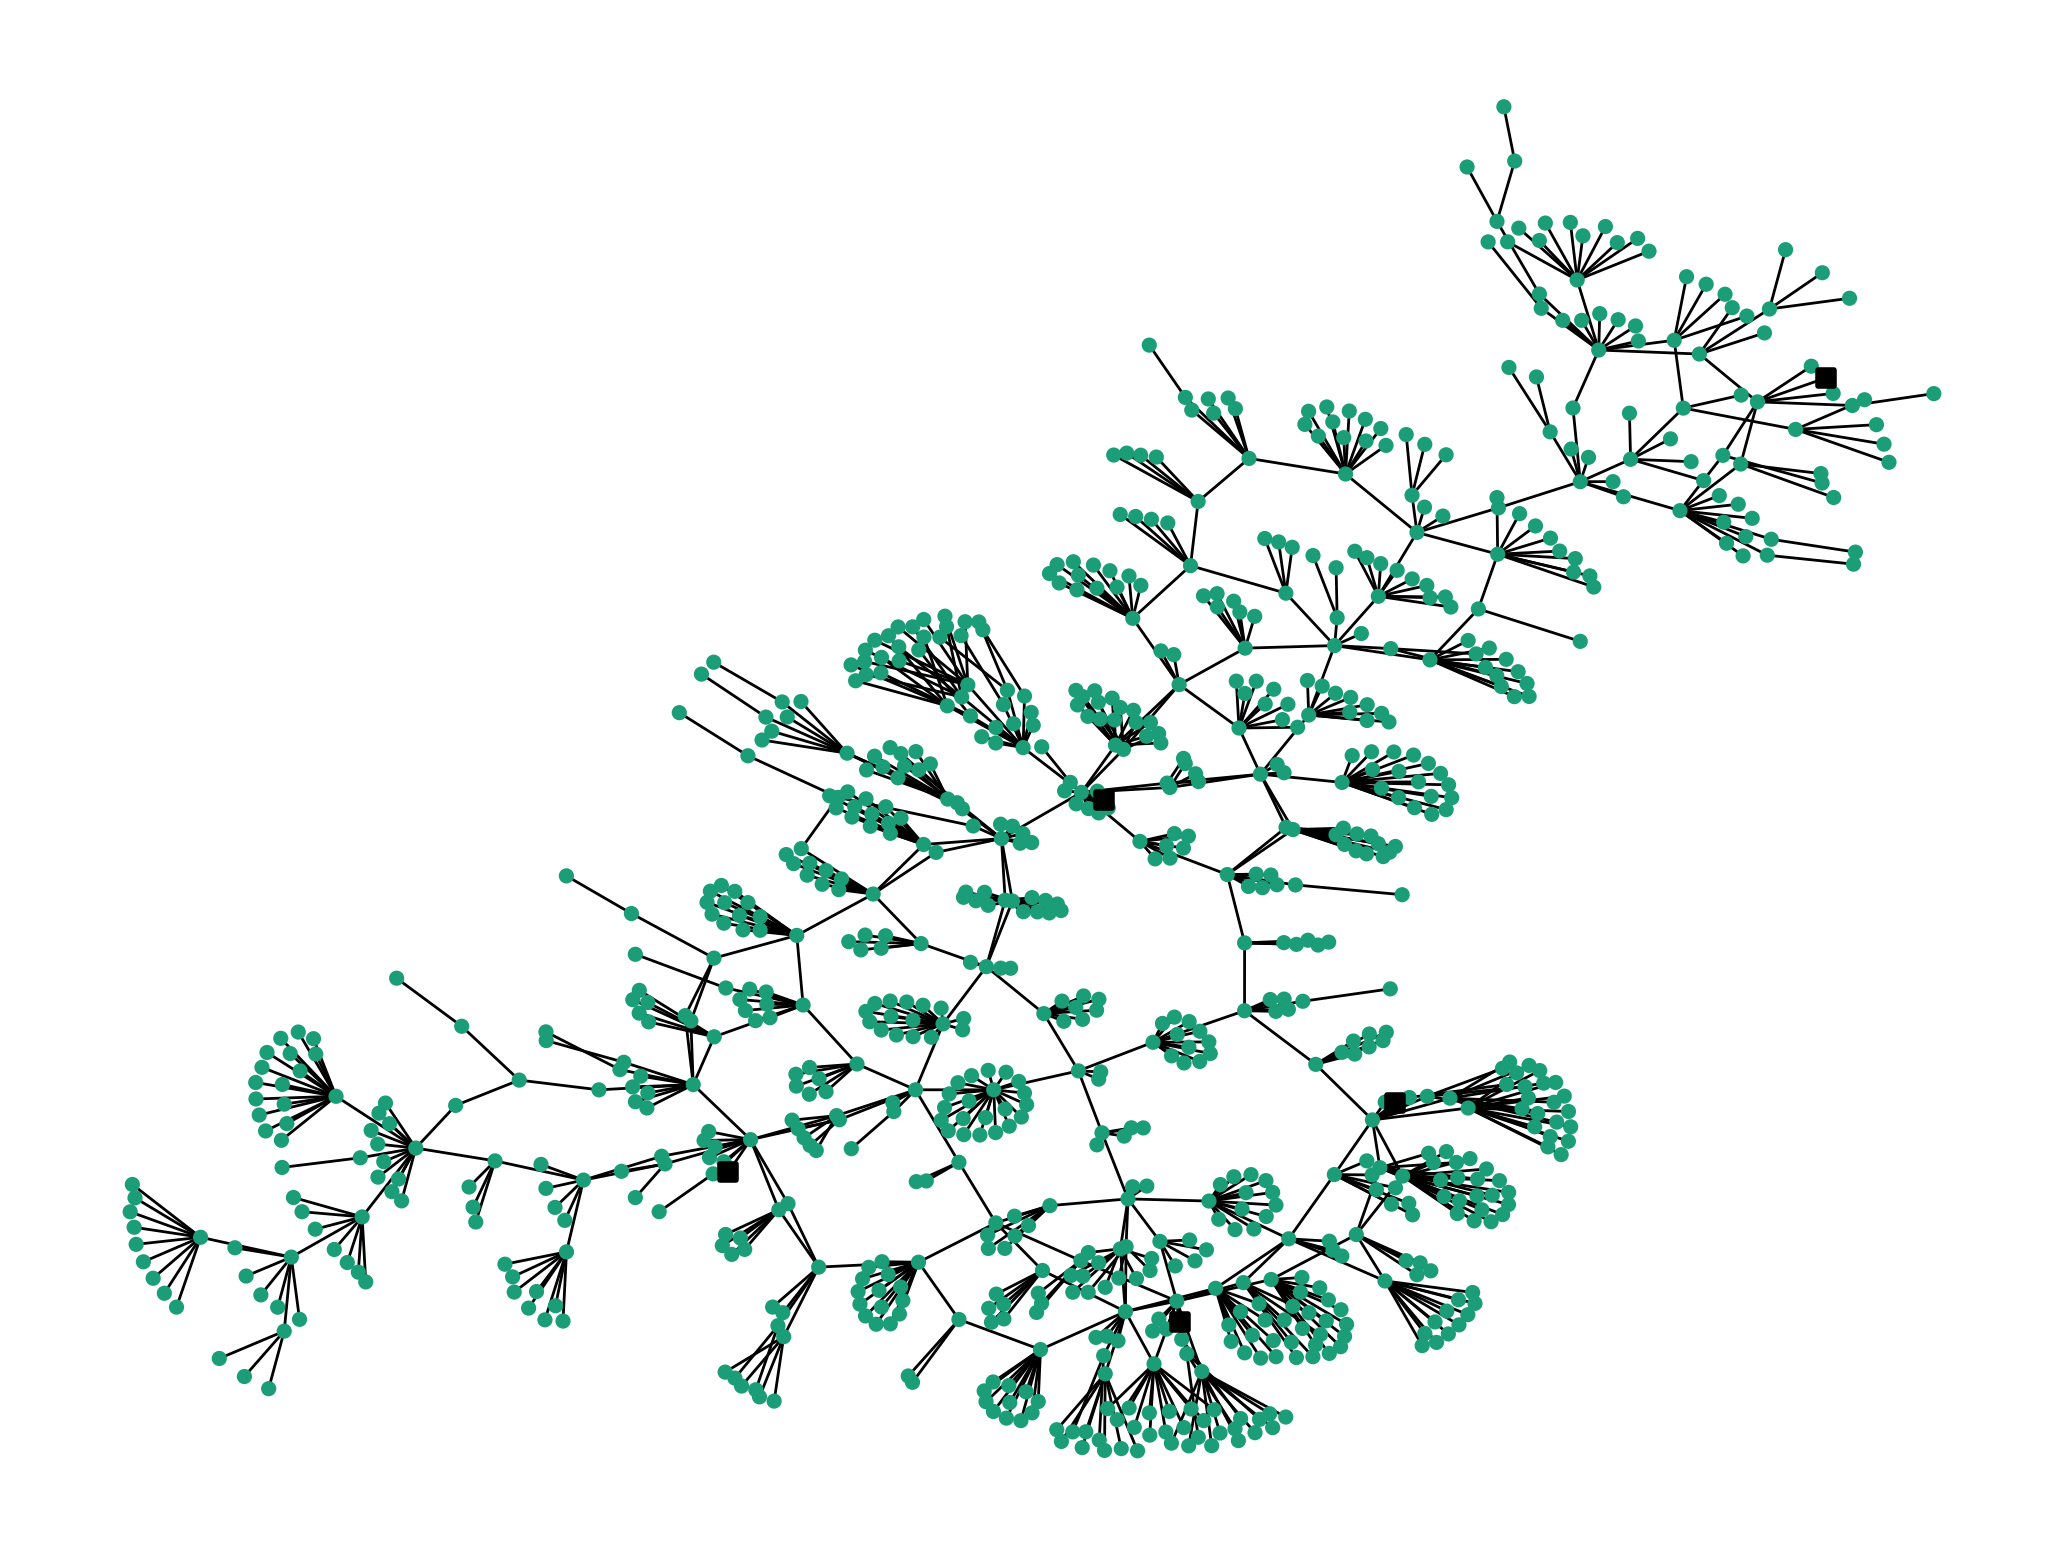
\includegraphics[width=.7\linewidth]{img/switchstate_exploring/swiss_suburb/topology_with_leafs.png}
    \end{center}
    \caption{
        Atomic islands formed out of swiss suburban grid data, laid out in a non-geographical way.
        Atomic islands shown as nodes with 
        ordinary islands in green and islands with transformers as black squares. Connecting switches between the
        atomic islands are shown as edges.
    }
    \label{fig:data_prep:swiss_suburb_with_leafs}
\end{figure}

From figure \ref{fig:data_prep:swiss_suburb_with_leafs} it can be seen, that
there are a lot of leaf nodes present. A leaf node is a node that only has
one connection in the graph structure. I.e. it is a "dead end" within the graph.
For switch state analysis these nodes are not interesting, as the switch leading
up to them can never be open as that would disconnect that leaf node and thus
disconnect the prosumers in that area.\\
This presents us with an opportunity to
reduce the number of nodes and connections needing to be examined further. Reducing the number of
nodes has considerable benefits later on as it speeds up any algorithm
searching through switch state possibilities. It also makes it visually clearer
what the switchable structure of the grid looks like. \\
We can get rid of the leaf nodes by merging them into their neighbouring nodes. 
After merging a leaf into its neighbour the resulting node might now be a leaf. Thus 
the leaf merging algorithm is repeated until there are no leaf nodes left. In the example
case this reduces the number of atomic islands by 801.

\begin{figure}[H]
    \begin{center}
        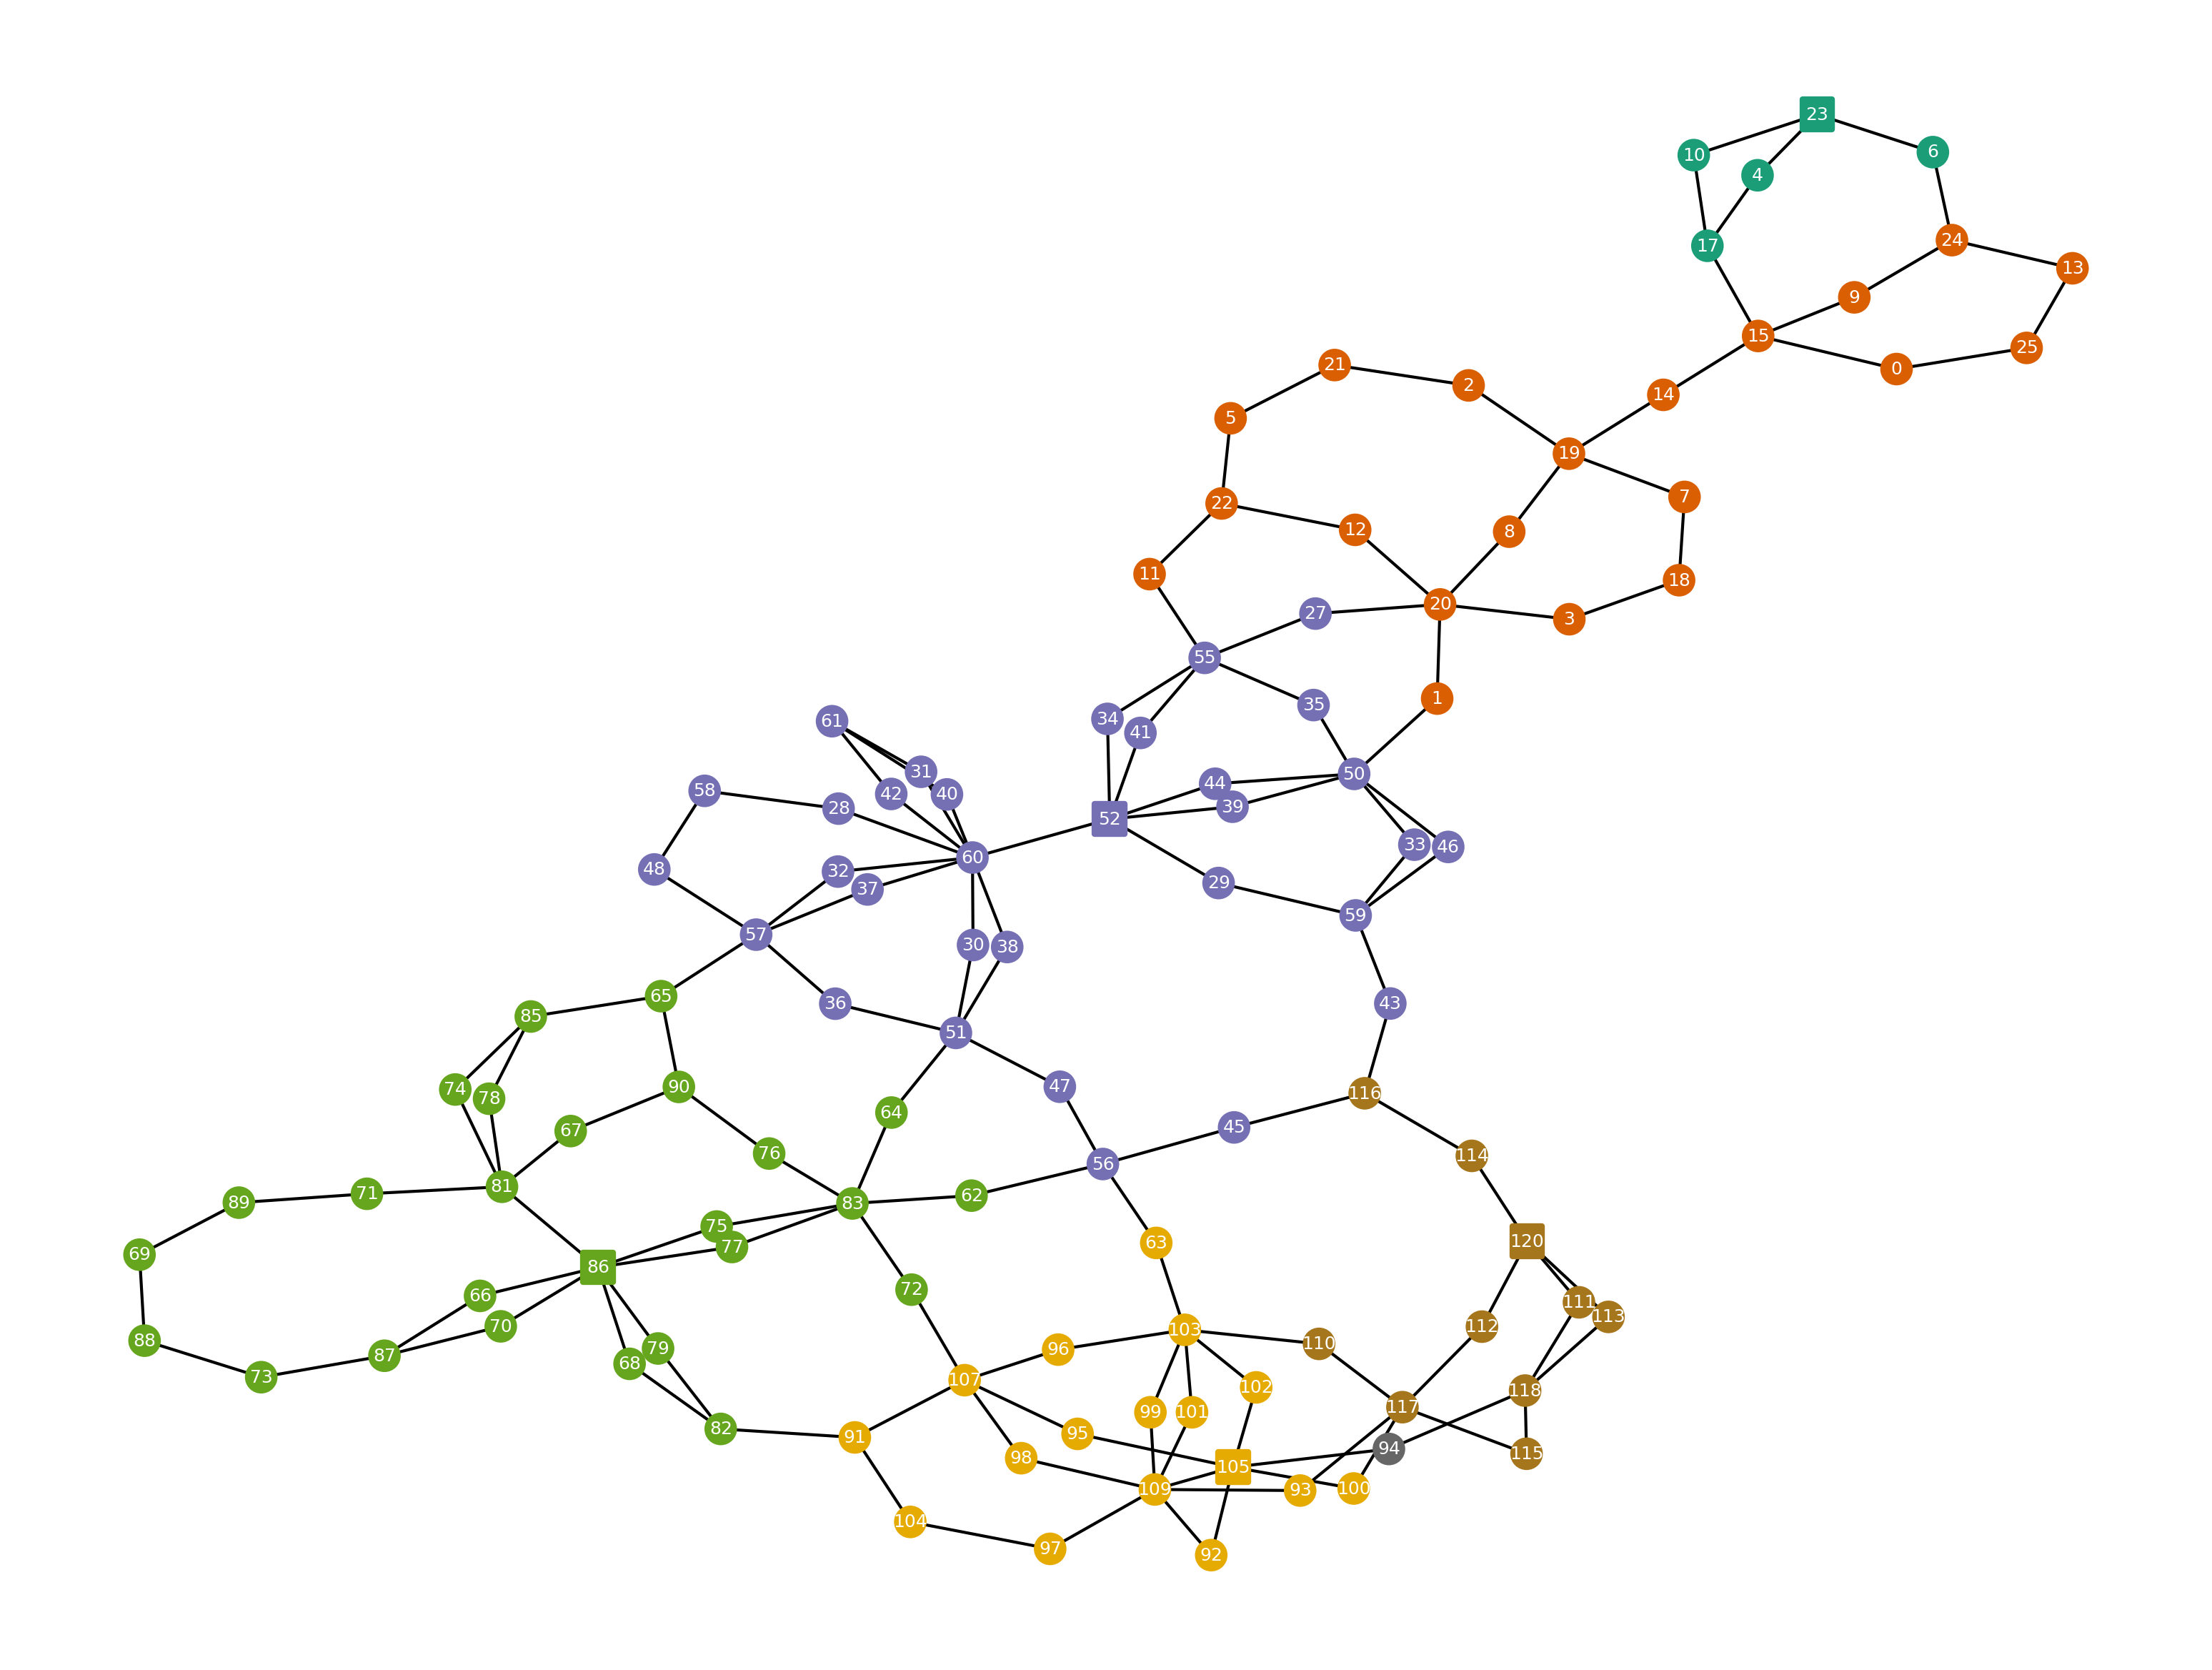
\includegraphics[width=.8\linewidth]{img/switchstate_exploring/swiss_suburb/topology_sss.png}
    \end{center}
    \caption{
        Atomic islands formed out of Swiss suburban grid data, laid out in a non-geographical way.
        Ordinary atomic islands shown as circles, atomic islands with transformer as squares. Atomic islands connected in the
        standard switch case shown as the same colour. Leaf atomic islands merged.
    }
    \label{fig:data_prep:swiss_suburb_topology}
\end{figure}

The last step in data preparation is to determine the standard switch state (SSS). The standard switch
state is the switch state that the grid is in if there are currently no faults or other abnormal
switching being done. I.e. it is the design switch state that the grid operator currently wants the
grid to be in. It is thus also reasonable to later compare any switch state changes to
the SSS and use it as a benchmark. To determine the SSS
an algorithm like algorithm \ref{alg:data_prep:atomic_islands} can be used again, with the nodes being
the atomic islands and the edges being all switches that are closed in the SSS.\\
\\
Lastly can be the case that there end up being atomic islands that are not connected to any
transformer in the SSS. This can happen if there is another neighbouring grid outwith the selected
geographical bounds or due to data quality issues. To rectify this atomic islands like these will
be merged into the island with the least overall grid load. This is to attempt and balance out
the load on the transformer and make the SSS perform the best it can. In the example
there are two clusters of unconnected atomic islands.
Node 94 (grey) and the orange cluster of nodes.
The result of merging them can be seen in \autoref{fig:data_prep:swiss_suburb_topology_patched}.

\begin{figure}[H]
    \begin{center}
        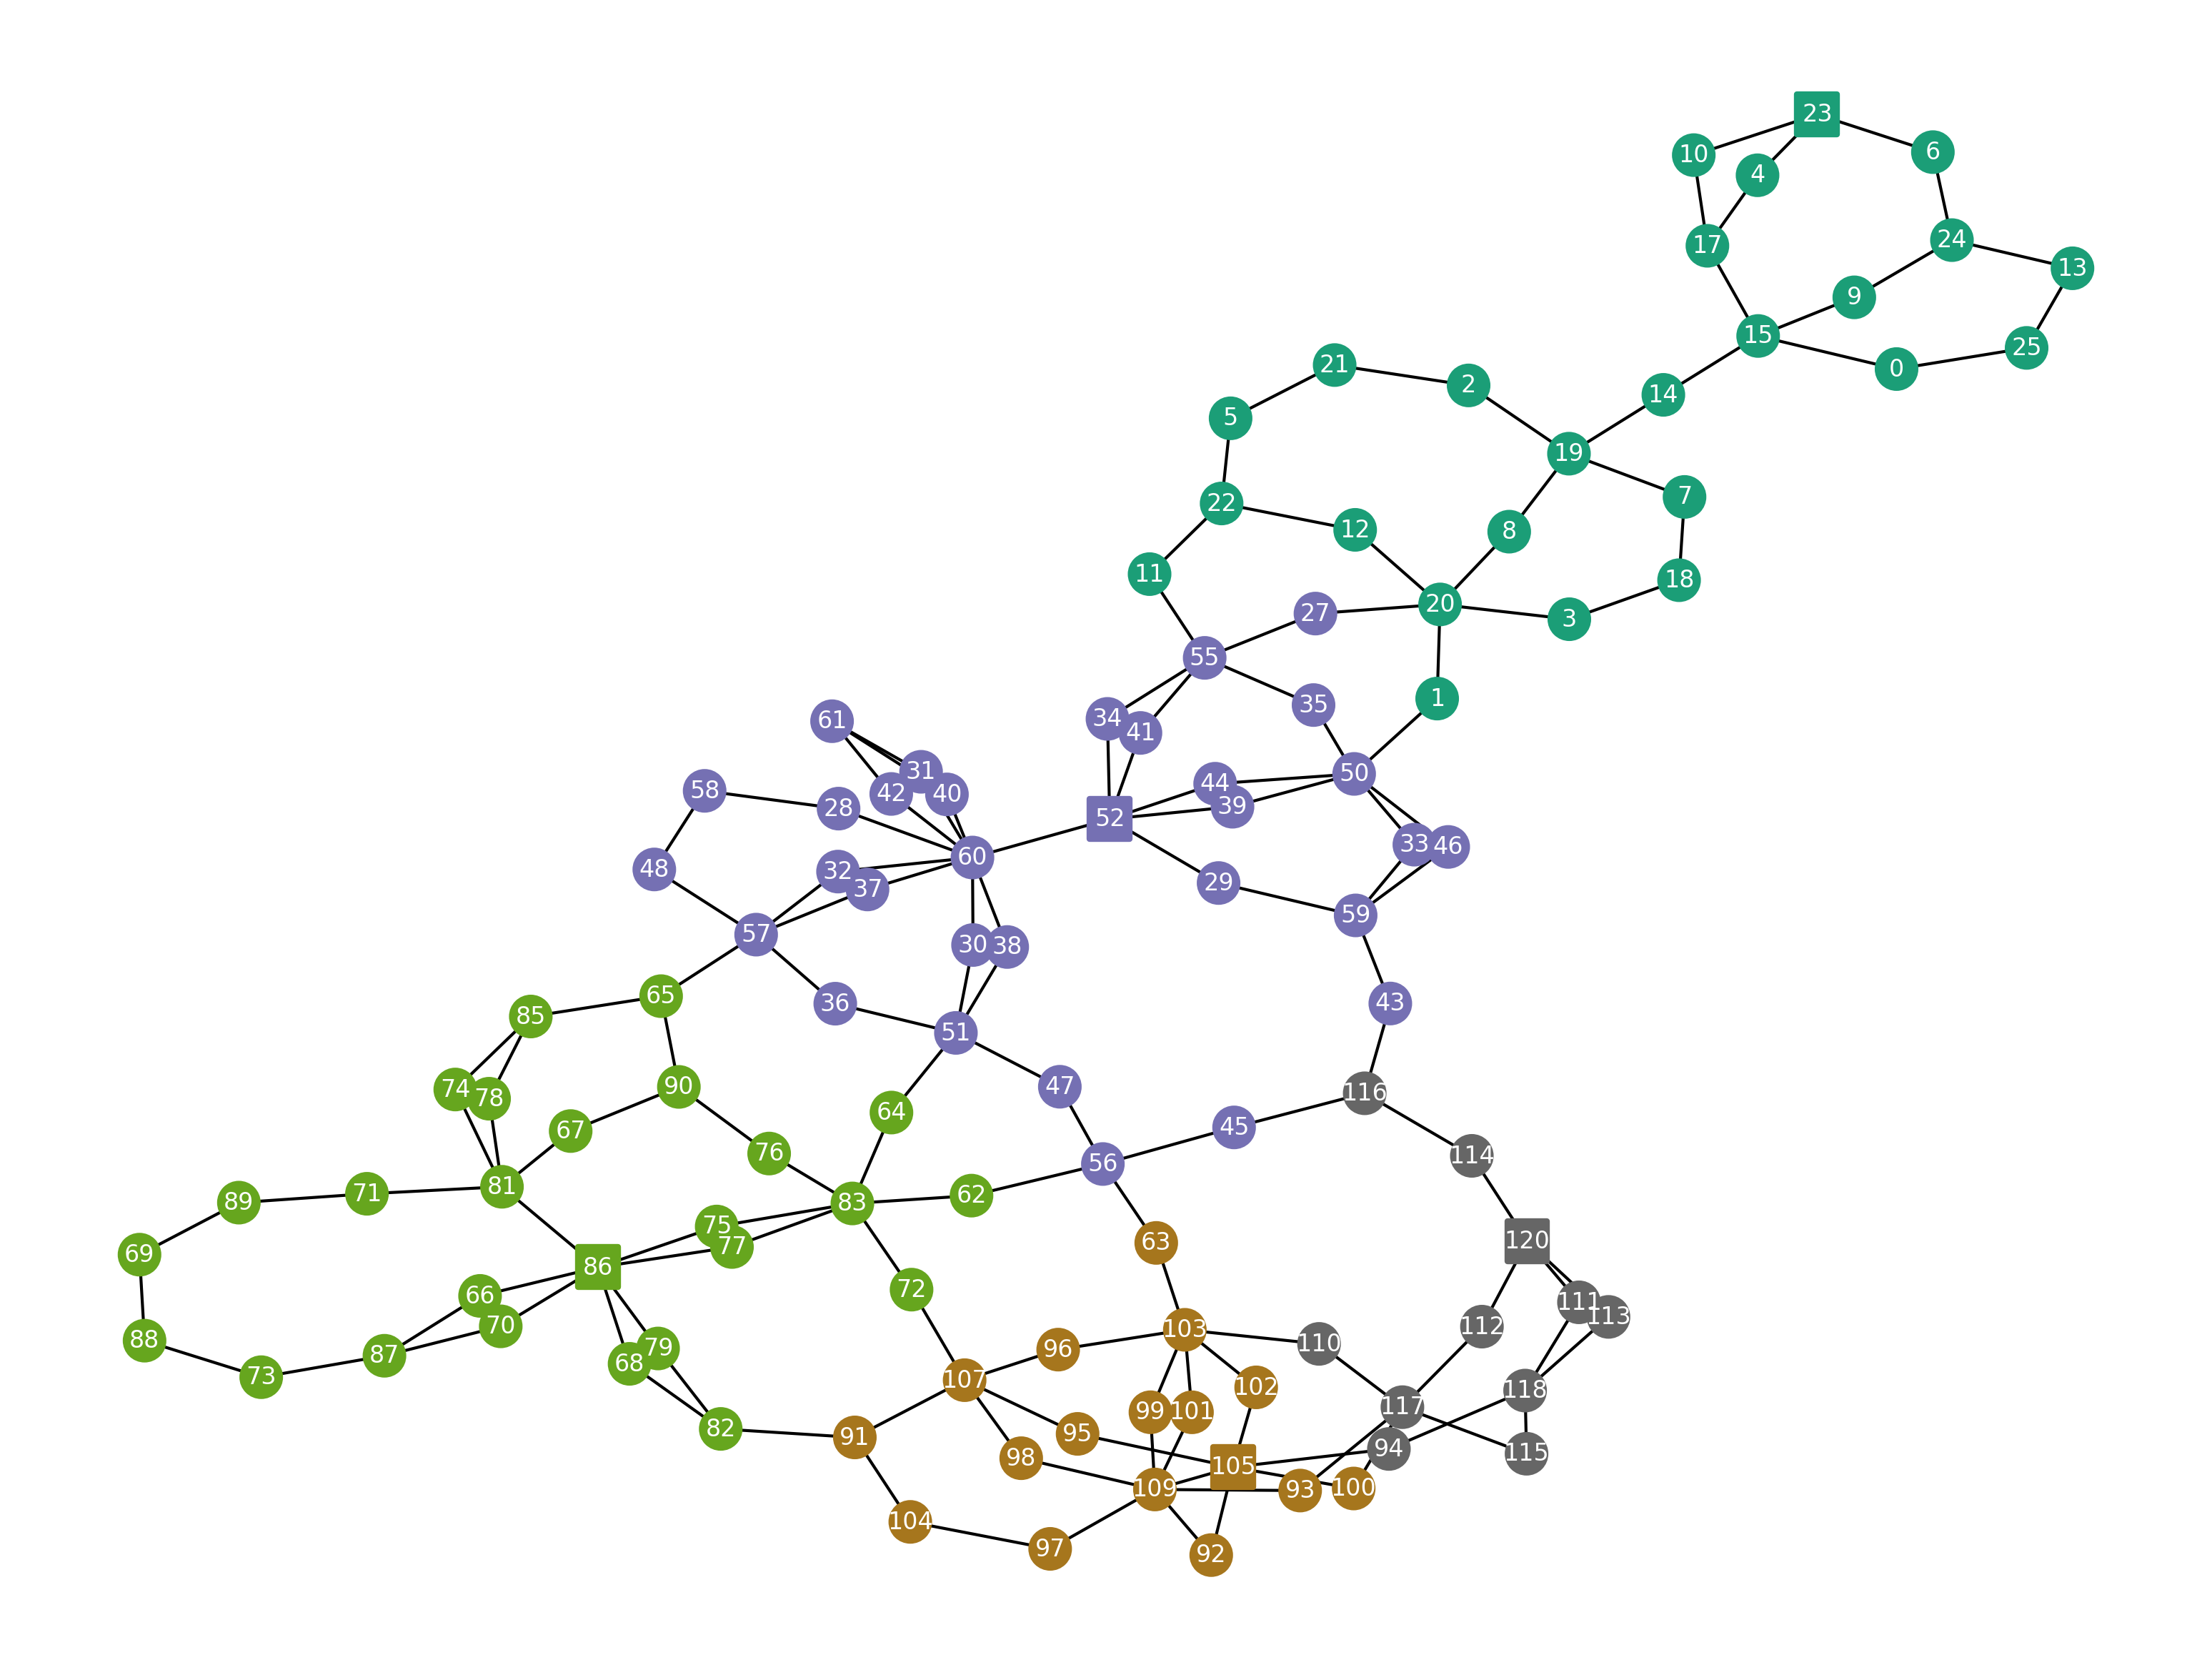
\includegraphics[width=.8\linewidth]{img/switchstate_exploring/swiss_suburb/topology_sss_patched.png}
    \end{center}
    \caption{
        Atomic islands from \autoref{fig:data_prep:swiss_suburb_topology} with unconnected islands
        connected to their neighbour with the lowest net consumption.
    }
    \label{fig:data_prep:swiss_suburb_topology_patched}
\end{figure}

\subsection{Powerflow}

% Mention how to prepare the data for powerflow